
The previous chapter presented the physical basis of the interactions between
hydrometeors and electromagnetic radiation, which cause an observable signal in
satellite observations. This chapter now turns to the problem of inverting this
signal to infer the physical properties of hydrometeors.


\section{The retrieval problem}
\label{sec:machine_learning:retrieval_problem}

Radiative transfer theory describes how radiation that propagates through the
atmosphere produces an observable electromagnetic signal. The that question
remains is how these observations can be used to derive estimates of physical
properties of the atmosphere. This is difficult because, although the
observations contain information on the hydrometeors in the atmosphere, they are
generally ambiguous, i.e.  two physically different atmospheric states can produce
the same observations, and affected by non-negligible measurement errors.

Mathematically, the problem of determining properties of hydrometeors from
satellite observations can be formulated as finding a state vector%
\footnote{% The notation for the state and observation vectors was deliberately
chosen to be the opposite of the conventions of inverse problem theory to make
it consistent with the conventions used in machine learning. }% $\vec{y} \in
\mathrm{R}^{n}$ that describes the physical properties of the atmosphere from a
vector of observations $\vec{x} \in \mathrm{R}^{m}$. This so-called
\textit{retrieval problem} can be solved using the mathematical framework of
inverse problem theory. In inverse problem theory, the underlying assumption is
that the observations $\mathbf{x}$ are generated by a physical processes, which
can be described using forward model function $f: \mathrm{R}^n \rightarrow
\mathrm{R}^m$, but may be affected by a random error $\mathbf{\epsilon} \in
\mathrm{R}^M$:
\begin{align}\label{eq:inverse_problem}
  \vec{x} &= f(\vec{y}) + \vec{\epsilon}
\end{align}

An exact solution to this problem does not exist. Because of the random noise
$\mathbf{\epsilon}$, the equation can never be strictly satisfied. Furthermore,
observations $\vec{y}$ of clouds are often ambiguous in the sense that a
physically different hydrometeor configuration, for example a cloud with more
and smaller particles, produces similar observations to another one. These
characteristics make the retrieval problem \textit{ill-posed}.

Although an exact solution to the retrieval problem is not possible, Bayesian
statistics can help us to extract the limited information in the observations
$\mathbf{x}$. In the Bayesian framework, both the observations $\vec{x}$ and the
atmospheric state vector $\vec{y}$ are assumed to be random variables.
Furthermore it is assumed that $\vec{y}$ is distributed according to a
known \textit{a priori} distribution $p(\vec{y})$. Instead of a single state
$\vec{y}$, the solution of the problem then becomes the posterior distribution
$p(\mathbf{y} | \mathbf{x})$ of the atmospheric state. According to Bayes
theorem, this solution is given by:
\begin{align}\label{eq:bayes}
  p(\mathbf{x} | \mathbf{y}) &= \frac{p(\mathbf{y}|\mathbf{x})
  p(\mathbf{x})}{p(\mathbf{y})}
\end{align}

Traditionally, Bayesian methods for solving the retrieval problem make use of
the right-hand side of Eq.~\ref{eq:bayes} to approximate the posterior
distribution. Instead of this, the approach pursued in this thesis is to learn
the posterior distributions $p(\vec{x}|\vec{y})$ directly from data. How this
can be done is the topic of the remainder of this chapter.

\section{Machine learning}


The field of machine learning is concerned with the development of algorithms
that can learn to solve computational tasks from data. More specifically, the
methods considered here solve the problem of \textit{supervised learning}. In
supervised learning the task is to learn how to produce outputs $y$ from
inputs $x$ given a set of pairs $\{(x_i, y_i)\}\text{ for }i = 1, \ldots, N$ of
specific inputs values $x_i$ and corresponding output values $y_i$. In general,
the inputs $x$ and outputs $y$ may represent anything from simple numbers to
images or texts. For the applications considered here, they inputs are typically
satellite images and the outputs corresponding physical quantities to be
retrieved.% as illustrated in Fig.~\ref{fig:machine_learning:input_output}.

Machine learning has gone through a wave of immense popularity during the 2010s
triggered by the success of \textit{deep learning} methods in addressing a range
of computational problems from the fields of computer vision, natural language
processing and artificial intelligence. The idea behind deep learning is to
construct increasingly powerful models by stacking a hierarchy of simple models.
Given sufficient data, these models can learn highly complex relationships and
require less guidance from human experts to achieve good performance.

\subsection{Shallow machine learning}

Although the focus of this thesis are deep learning methods, this section will
use a very shallow model to illustrate the basic principles of machine learning
based retrievals. We consider the example of estimating rain at the surface from
infrared observations ($\lambda = \SI{10.3}{\micro \meter}$). The data that is
used to train the retrieval model consists of co-located observations of the
geostationary satellite and combined radar/micowave radiometer retrievals.

In this particular case the input $x$ corresponds to the measured radiation at a
single pixel of the geostationary observations and the output $y$ to the rain rate
that is to be estimated from the satellite observations. To so, a linear regression
model is used to relate the observations $x$ to the rain rate:
\begin{align}
  y &= a x + b
\end{align}
The two parameters of the model are the slope $a$ and the intercept $b$.
They can be determined by finding the values, which minimize the
squared error between the estimates and the true values on the training data.

Panel (a) in Fig.~\ref{fig:machine_learning:linear_regression} shows the
distribution of the training data together with the learned relationship between
input and output data. This view reveals already that the relationship is not
very robust, which becomes even clearer when the retrieval results (Panel (b))
are compared to the reference precipitation (Panel (c)). The linear regression
model simply predicts rain almost everywhere there is a high cloud. Although
this may be a good guess in the absence of additional information, this simple
model completely fails to reproduce the structure in the reference
precipitation.

\begin{figure}
  \centering
  \includegraphics[width=\textwidth]{linear_regression.png}
  \caption{Example of a very simple precipitation retrieval. Panel (a) shows a density
    plot of the distribution of the input-output pairs, which consist of IR brightness
    temperatures and surface precipitation rates. The white line show the
    log-linear relationship between obtained by linear regression. Panel (b) shows
    retrieved precipitation rates when the learned relationship is applied to
    real observations. Panel (c) shows the true precipitation rates as present
    in the training data. Note that due to the nature of the co-locations the precipitation
    is not know across the full scene.
  }
  \label{fig:machine_learning:linear_regression}
\end{figure}

Given the bad performance of the simple linear regression model, the question
how can a better retrieval model be obtained? In general there are three
dimensions along which a machine learning model can be improved:
\begin{description}
\item[Model expressivity:] The model used in this example can only learn
  linear relationships between input and output. The range of mathematical functions
  that a model can represent is referred to as its \textit{expressivity}. Increasing
  the model expressivity, enables it to learn  more complex relationships between
  the input and output.
\item[Amount of input information:] The scatter plot in
  Fig.~\ref{fig:machine_learning:linear_regression} shows the problem of
  retrieving precipitation from IR observations is highly degenerate. For any
  value of the observations, training data contains different precipitation
  values, which makes it impossible to assign a unique 'right' precipitation
  rate to an observed brightness temperature. The degeneracy can be decreased by
  adding more information to the input. This can be achieved, for example, by
  adding observations from other channels or information from neighboring pixels
  in order to give the model more flexibility to distinguish different
  precipitation rates.
\item[Amount of data:] A machine learning model can only learn relationships
  that are sufficiently well represented in the training data. For more complex
  retrievals than this one, larger amounts of training data are crucial for good
  retrieval performance.
\end{enumerate}

Traditionally, the difficulty in improving a machine learning model was that it
is not sufficient to just increase the model expressivity or the amount of input
information. Since both measures increase the flexibility of the model, they may
cause it to \textit{overfit} on the training data. Overfitting occurs when the
model learns spurious relations from the training data, which are not actually
representative of the true relationship between input and output. This typically
causes predictions on unseen data to deteriorate drastically. Overfitting can be
counteracted by artificially reducing the expressivity of the model, a process
that is called \textit{regularization}, and by increasing the amount of data
that is used to train the model. However, the time and computational resources
that are required for training typically increase with the amount of data. If
the this increase is too rapid, the amount of data that a machine learning model
can be trained on may be limited.

Machine learning models therefore traditionally depended on careful tuning to
the task at hand. Especially the trade-off between model expressivity and the
amount of data that can be used to train the model required a multi-disciplinary
approach that combined domain-specific knowledge with machine-learning
experience to develop a good-performing model. A particular difficulty of
shallow models was their inability to handle large inputs with low information
content such as all pixels from an image, which made the models prone to
overfitting and harder to train. This gave rise to the practice of
\textit{feature engineering}, which consists of manually designing input
variables that encode more useful information in a smaller number of inputs.

It should be noted here that the linear-regression model used here is extremely
simple and that there are shallow machine learning methods, which can would work
much better the precipitation. Nonetheless, the example is not totally
unrealistic given that it is similar to early precipitation retrievals from
geostationary observations \citep{vicente98}. To overcome the limitations of the
linear regression, the model from \citet{vicente98} predicts precipitation in
log-space and uses weather model data to post-process the retrieval results.
Modified version of this retrieval are still in operational use today
\citep{siqueira19}.

\subsection{Deep learning}

The example discussed above demonstrated the limitations of very shallow
machine learning methods. But how can deep learning help to overcome these
limitation?

The essential promise of deep learning is that it decouples the dimensions along
which a machine learning model can be improved. This is achieved primarily by
scalability. Deep learning models achieve high expressivity by stacking a large
number of simple models. The training time of deep learning methods scale
linearly with the amount of available data, while the required memory remains
constant. By balancing the increased model expressivity with large amounts of
training data, these models can learn highly complex relationships without
seriously overfitting.

  \subsection{Neural networks}

  The basic idea of deep learning is to construct expressive models by stacking
  simple models. The simple linear regression model from above can be extended
  to a deep model by replacing the simple linear regression that predicts a
  single value $y$ from a value $x$ with multi-variate multi regression, which
  produces an intermediate vector $\vec{y}_1$ from an input vector
  $\vec{x}$. The multi-variate regression transform of the input vector
  $\vec[x}$ into the vector $\vec{y}_1$. Its specific form is determined by the
  values of the coefficients of the multi-variate multi regression.

  A neural network is just a sequence of consecutive, parametrized
  transformations, which are referred to as \textit{layers}. Each of these
  layers transforms an input vector into an output vector and its exact form
  can be adapted by modifying its parameters. Just as in the case of linear
  regression these parameters can be learned by minimizing an error metric
  over the training data.

  An important characteristic of this definition of a neural network is its
  recurrence: A neural network is itself a transformation of an input vector
  into an output vector and may thus be used as a layer in a larger network. At
  the same time, however, this makes the defintion of what exactly constitutes a
  layer in a network somewhat arbitrary.

  \subsubsection{The multi-layer perceptron}

  The multi-variate multiple regression layer introduced above constitutes one of
  the most fundamental transformations for neural networks. It is typically
  referred to as a fully- or densely-connected layer. Mathematically, this layer
  implements an affine transformation of the input vector $\bm{x}$ of the form
  \begin{align}
    \bm{y} = f(\bm{x}) = \bm{W}x + \bm{b}
  \end{align}
  where $\bm{W} \in \mathrm{R}^{m \times n}$ is a matrix of weights $W_{i,j}$
  for $i = 1, \ldots, m$ and $j = 1 \ldots n$ and $\bm{b}$ a vector of offsets
  or biases $b_i$ for $i = 1, \ldots m$.

  Fully-connected layers are typically paired with a non-linear function, which
  is applied element-wise to the its outputs. This is because without these
  non-linear activation functions, stacking of fully-connected layers does not
  increase their expressivity, which in this case depends only on the number of
  input and output variables.

  There exist a wide range of activation functions. One of the currently most
  commonly used activation function in deep networks is the Rectified Linear
  Unit (ReLU).
  \begin{align}
    \text{ReLU(x)} = \begin{cases}
      x & x > 0 \\
      0 & x \leq 0
    \end{cases}
  \end{align}
  It should be noted, however, that neural network architectures are an active area of
  research and several alternatives and modifications of the ReLU activation have
  been proposed.

  A neural network which consists of one or several layers of fully-connected
  layers followed by activation functions is typically referred to as
  multi-layer preceptron (MLP). Since all numeric inputs can be brought into
  vector form and thus fed into an MLP, the MLP is one of the most fundamental
  forms of neural networks.

\subsubsection{Convolutional neural networks}

Although MLPs can in principle be applied to image data directly by flattening
the input data into a single vector, this approach was found to not work well in
practice. The reason for this that the number of parameters in the model becomes
very large, which makes the model sensitive to overfitting and the training more
difficult.

An important technique in the application of neural networks to image data, was
the introduction of the convolutional layer, which replaces the
matrix-multiplication of the fully-connected layer with a convolution with a
learnable filter kernel. Let $\bm{X} = X_{i, j}$ for $i = 1, \dots, M, j = 1,
\ldots, N$ be an input image of size $M \times N$. Given a kernel $\bm{K} =
K_{i, j}$ for $i = 1, \ldots, k, j = 1, \ldots, k$, the convolution $\bm{Y} =
\bm{X} * \bm{K}$ of $\bm{X}$ and $K$ is defined as
\begin{align}
  Y_{i, j} &= \sum_{l=-k}^{k} \sum_{m=-k}^{k} X_{i + l, j + k} K_{i - l, j -k}
\end{align}
The convolution can be visualized as a constant filter mask that is shifted over
the input image to generate an output image. Since the convolution
transformation is linear, it is a special case of the fully-connected
transformation of the corresponding flattened input image.

The convolution operation can  be seen as a restriction of the more general
fully-connected layer, which encodes two important properties of images into the
neural network model: Translation invariance and locality. Translation
invariance refers to the fact that the output of the convolution operation is
independent of the relative location within the image. It is easy to see that
this is a very suitable assumption for object detection tasks, since the way an
object looks is not affected by its position in the image. The property of
locality refers to the face that the output of a convolution layer is determined
only by a limited, connected subset of pixels of the input image, the number of
which depends on the kernel size $k$. This thus encodes the assumption that for
understanding the content of a given image region, neighboring pixels should
have larger relevance than those further away.

To allow convolutional neural networks to combine information across different
image scales, these layers are typically combined with downsampling layers that
successively decrease the size of the input image. The motivation for this is to
allow the model learn a hierarchy of transformations from the large amounts of
low-level information on the pixel scale to a reduced amount of high-level
information, which is relevant for the task at hand.

\subsubsection{Training}

Now that the basic building blocks of modern neural networks have been
introduced, the question remains how they can be trained to solve a given
computational task. As mentioned above, we are considering the case of
supervised learning in which training data in the form of samples from the joint
distribution of input data $x$ and corresponding outputs $y$ are available.

The basic training approach is the same as the fitting of the parameters of a
linear regression model, which are found by minimizing a certain loss criterion
over the training data. For linear regression this is typically the mean squared
error, which  can also be used to train neural networks. In contrast to linear
regression, however, the parameter optimization of for the neural network can
not be solved explicitly. Instead, neural networks rely on iterative training by
minimizing the loss function using gradient descent optimization.

While naive gradient descent would require traversing the whole training dataset
to compute the gradients to perform a single gradient descent step, it is in
practice sufficient and even beneficial to only use a small subset of samples
from the training data. This modification of traditional gradient descent, which
is known as stochastic (mini-batch) gradient descent allows neural network to
scale efficiently to very large datasets. In addition to that, the stochasticity
of the calculated gradients prevents the optimization process from getting stuck
in local minima of the cost function.

\subsubsection{Uncertainty in machine learning}

The ill-posed character of the retrieval problem discussed in
\ref{sec:machine_learning:retrieval_problem} leads to significant
uncertainties in most remote sensing retrievals. In addition to that,
the machine learning approach gives rise to two additional source
of uncertainties in the retrieval.

%Machine learning techniques allow us to train a model that retrieved physical
%quantities from satellite observations. However, as discussed in
%Sec.~\ref{sec:remote_sensing:retrieval_probem}, there is no unique solution to
%the retrieval problem. Mathematically, this means that any prediction consisting
%of just a single value will always be wrong. Given the impossibility of solving
%the retrieval problem exactly and import question becomes whether the model
%learn how wrong it is?

The total error that a machine learning model makes in its prediction is ts
\textit{predictive uncertainty}. The predictive uncertainty can be decomposed
into three independent sources. The first one, referred to as \texit{epistemic
  uncertainty}, is uncertainty caused by a lack of training data. Its defining
property is that this uncertainty can be reduced by collecting more data to
train the model. The second type is called \textit{aleatoric uncertainty}. This
uncertainty refers to the uncertainty that cannot be reduced by increasing the
amount of data that the model is trained on. In the context of satellite
observations this uncertainties is caused by the inability of the observations
to fully determine the observed atmospheric state. It is thus a consequence of
the ill-posed nature of the retrieval problem as discussed in
Sec.~\ref{sec:remote_sensing:retrieval_problem}.
The final type of uncertainties is caused by differences between the training
data and the data that the model is actually applied on. It is typically
referred to as \textit{covariate shift}. It is obvious that when the wrong data
is used to train the model it is likely to produce wrong results. However,
subtle changes between training data and the actual data that the model is
applied to are not uncommon and can thus increase the predictive uncertainty of
the model.

\section{Handling uncertainty in remote sensing retrievals}

One of the issues that the work presented in this thesis aims to address is the
quantification of retrieval uncertainties in machine-learning-based remote
sensing retrievals. The two methods that were explored in the appended studies
can be categorized as probabilistic regression approaches. This means that they
account for the aleatoric uncertainty in the prediction but neglect epistemic
uncertainty and covariate shift. Below, these two approaches are presented
followed by a discussion of other approaches to quantifying uncertainties in
remote sensing retrievals.

\subsection{Probabilistic regression}

Aleatoric uncertainty arises due to ambiguous samples in the training data. The
fact that these ambiguities are represented in the training data means that they
can be predicted by a suitably trained neural network model. To allow for this,
the deterministic formulation of regression, i.e. to predict a single value $y =
f(x)$, is replaced by the probabilistic formulation to predict the probability
distribution $p(y|x)$ of $y$ given the input $x$.

\subsubsection{Quantile regression neural networks}

%To predict a distribution $p(y|x)$ the neural network model can trained
%to predict parameters of a parametrized probability distribution and
%an optimization criterion for the training can be obtained by maximizing the
%likelihood of the training samples under the predicted distribution. Assuming
%$p(y|x)$ to be Gaussian distributed with mean $\mu = f(x)$ and constant standard
%deviation yields a training criterion equivalent to the MSE loss.

Quantile regression neural networks (QRNNs) predict the distribution $p(y|x)$
for scalar output $y$ using a sequence of its quantiles.


Given a fraction $\tau \in [0, 1]$, the corresponding quantile $y_\tau$ is
defined as
\begin{align}
  y_\tau &= F^{-1}(\tau)
\end{align}
with $F(y) = \int_{-\infty}^y p(y|x)\ dy$ the cumulative distribution
function (CDF) of the distribution $p(y|x)$. A neural network can learn to predict a quantile
$y_\tau$ by training it to minimize the quantile loss
\begin{align}
  \mathcal{L}(y_\tau, y) &=
  \begin{cases}
    \tau  |y_\tau - y| & \text{if } y > y_\tau \\
    (1 - \tau)  |y_\tau - y| & \text{otherwise} \\
    \end{cases}
\end{align}
where $y_\tau$ is the predicted quantile and $y$ is the reference output value
from the training data. What is important to realize here is that $y$ is only
required to be an an ordinary sample of the distribution $p(y|x)$, i.e. the output
value corresponding to the input $x$.

This approach can be extended to multiple quantiles corresponding to
a sequence of quantile fractions $\mathrm{T} = \{\tau_1, \ldots, \tau_N\}$ by training
the network to minimize the sum of the quantile losses
\begin{align}
  \mathcal{L}_\mathrm{T}(\vec{y}_T, y) &= 
  \sum_{\tau \in \mathrm{T}} \mathcal{L}_\tau(y_\tau, y)
\end{align}
where now $\vec{y}_T = [y_{\tau_1}, \ldots, y_{\tau_N}]$ is a vector of predicted quantiles.

The basic functioning of neural networks is illustrated
Fig.~\ref{fig:machine_learning:qrnn}. To predict the distribution of a scalar
variable $y$ conditioned on a vector of inputs $\vec{x}$, QRNNs use a neural
network to transform the vector of inputs into a vector of outputs. The outputs
correspond to a sequence of quantiles, which can be used to derive a piece-wise
linear approximation of the CDF of $p(y|x)$.

\begin{figure}[btp]
  \centering
  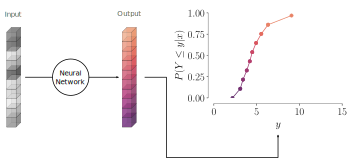
\includegraphics[width=.75\textwidth]{qrnn.pdf}
  \caption{The basic functioning of QRNNS. QRNNs predict the distribution of
    a scalar output variable $y$ using a vector of quantiles from which the
    an approximation of the CDF of the distribution can be constructed.}
  \label{fig:machine_learning:qrnn}
\end{figure}

Using quantile to represent the distribution $p(y|x)$ has the advantage that the
neural network can learn the shape of the output distribution. This is in
contrast to other probabilistic regression methods, which often impose a more
constrained parametrized form of $p(y|x)$ such as a Gaussian whose mean and
standard deviation are predicted.

An unresolved issue with QRNNs are crossing quantiles. In the form employed
here, there is nothing that ensures that the predicted quantiles are increasing.
QRNNs can thus produce mathematically inconsistent predictions. 
Since in practice usually only a limited number of quantiles or derived statistics
are likely to be stored as retrieval output, this was not found to be a critical
limitation QRNNs.


\subsubsection{Density regression neural networks}

The second approach for predicting the distribution $p(y|x)$ is based the work
by \citet{oord16} and \citet{sonderby20}. Since the approach has been given an
explicit name by the authors, we refer to it as density regression neural
networks (DRNNs) here. For this approach the regression problem is cast as a
classification problem by discretizing the domain of output values $y$ into bins
$y_0, \ldots, y_n$ and then predicting for each bin the probability
$p_i(Y >= y_{i - 1}, Y < y_i)$ of the observed $y$ falling into the $i$th bin.


Mathematically this is implemented by minimizing the
categorical cross entropy loss
\begin{align}
  \mathcal{L}(\hat{\vec{y}}, y) &=  -\log(\hat{y}_i) \text { with i s.t. } y_{i - 1} \leq y < y_i.
\end{align}
where $\hat{\vec{y}} = [y_1, \ldots, y_n]$ is a vector of predicted probabilities.

The predicted vector of bin probabilities can then be used as a piece-wise
constant approximation of the PDF of $p(y | x)$, as illustrated in
Fig.~\ref{fig:machine_learning:drnn}. Since the CDF of $p(y | x)$ can be
calculated from the PDF and vise versa, QRNNs and DRNNs are functionally very
similar. Compared to QRNNs, DRNNs have the advantage of avoiding quantile
crossing by construction. What may be disadvantage of DRNNs is that they require
a relative large output vector when values of $y$ vary over multiple orders of
magnitude.

\begin{figure}[btp]
  \centering
  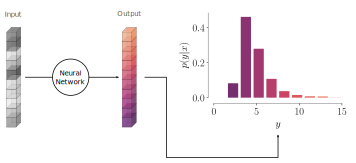
\includegraphics[width=.75\textwidth]{drnn.pdf}
  \caption{The basic functioning of QRNNS. QRNNs predict the distribution of
    a scalar output variable $y$ using a vector of quantiles from which the
    an approximation of the CDF of the distribution can be constructed.}
  \label{fig:machine_learning:drnn}
\end{figure}

\subsubsection{The aleatoric approximation}

Both QRNNs and DRNNs only learn to quantify the aleatoric uncertainty and
neglect epistemic uncertainy and covariate shift. For these models to produce
reliable uncertainty estimates, it is therefore necessary that the aleatoric
component of the predictive uncertainty dominates the two other types of
uncertainties. This assumption can be justified considering the remote sensing
observations are produced in a controlled environment and the range of possible
observations is generally well understood. Besides that, given the cost of
designing and operating these observation systems, it should be the aim to
minimize both epistemic uncertainty and covariate shift, which leaves the
aleatoric uncertainty as the only irreducible source of uncertainty in the
predictions.

Additional, empirical evidence for the usefulness of the aleatoric approximation
comes from the results presented in this thesis. In the applications considered
there, the probabilistic predictions from QRNNs and DRNNs provide reliable
estimates of the retrieval uncertainty.

%\subsubsection{Limitations}
%
%In addition to being limited to predicting the aleatoric uncertainty,
%QRNNs and DRNNs are incapable of modeling correlations between multiple
%output variables. This means that these methods are incapable of generating
%realistic spatial fields representing samples from the joint distribution
%of the output variables.

\subsection{Other approaches for quantifying uncertainties}

The two principal limitations of the QRNNs and DRNNs are that they can only
quantify aleatoric uncertainty and that they cannot be used to model correlation
between multiple output variables. Because of this, they may not be the best
choice for all applications. We therefore briefly review other approaches for
quantifying retrieval uncertainty and compare them to the probabilistic
regression approach.

\subsubsection{Bayesian neural networks}

Bayesian neural networks (BNNs) can handle both epistemic and aleatoric
uncertainty. For BNNs not only the target $y$ is assumed to be a random variable
but also the parameters $\theta$ of the neural network model. The distribution
of these parameters describes the uncertainty in the training of the model,
which is caused by the finite amount of training data.

The model predicts the distribution $p(y|x, \theta)$ of the target $y$ given
input $x$ and a realization of model parameters $\theta$. The epistemic
uncertainty in the model predictions can be quantified by sampling multiple
instances of the model parameters $\theta$. For inputs $x$ that the model has
encountered often during training, the distribution of $\theta$ values will be
such that $p(y|x, \theta)$ does not change much for different realizations of
$\theta$. For samples where this is not the case, there will be more spread in
the predictions.

Despite their ability to quantify both aleatoric and epistemic uncertainty, BNNs
have not yet found widespread adoption for practical machine learning
applications. One reason for this is likely that their training takes
significantly more time. Another disadvantage is that the quantification of
epistemic uncertainty requires evaluating the network multiple times. Since
this increases the time required to evaluate the model by an order of magnitude,
this may be a disadvantage for applications that produce large amounts of
data or are time-critical.

Despite these potential disadvantages, \citet{orescanin22} have recently
demonstrated the application Bayesian neural networks to the classification of
precipitation types and shown that the predicted uncertainties are well
calibrated. They also found that the predictive uncertainty is dominated by
aleatoric uncertainty, which thus provides further evidence for the
validity of the aleatoric approximation.

\subsubsection{Generative models}

Another approach to quantify uncertainties in neural network predictions are
generative models. Instead of predicting the conditional probability
distribution $p(y|x)$ explicitly, these methods are trained to directly generate
samples from the distribution. These methods have gained popularity in computer
vision tasks due to their ability to generate samples from highly complex
probability distributions such as images of faces or generic objects. The
advantage of this approach is that it can handle spatial correlations in the
uncertainties, which is not the case for the two other approaches discussed
above.

What makes generative models interesting is their ability to represent
correlations between output variables in the samples they generate. Recent work
has explored the application of generative models for short-term weather
forecasting \citep{ravuri21} and probabilistic downscaling of precipitation.
However, these models are also more difficult and expensive to train than
standard neural network and require multiple evaluations during inference.
